\chapter{Applications of Double Integrals}

\section{Total Mass and Charge}
Suppose there is a generic, thin layer (called a \textit{lamina}) with a 
variable density that occupies an area \textit{B} (see figure \ref{fig:lamina}).
Further, let the density of the lamina be described by a function, $\rho 
(x, y)$, which is continuous over \textit{B}. For some small rectangle centered
at $(x, y)$, the density is given by:
$$\rho (x, y) = \frac{\Delta m}{\Delta A}$$

Where $\Delta m$ is the mass of the small rectangle and $\Delta A$ is the area.
Then the mass of the rectangle is given by:
$$\Delta m = \rho (x, y) \Delta A$$

\begin{figure}[htbp]
\centering
    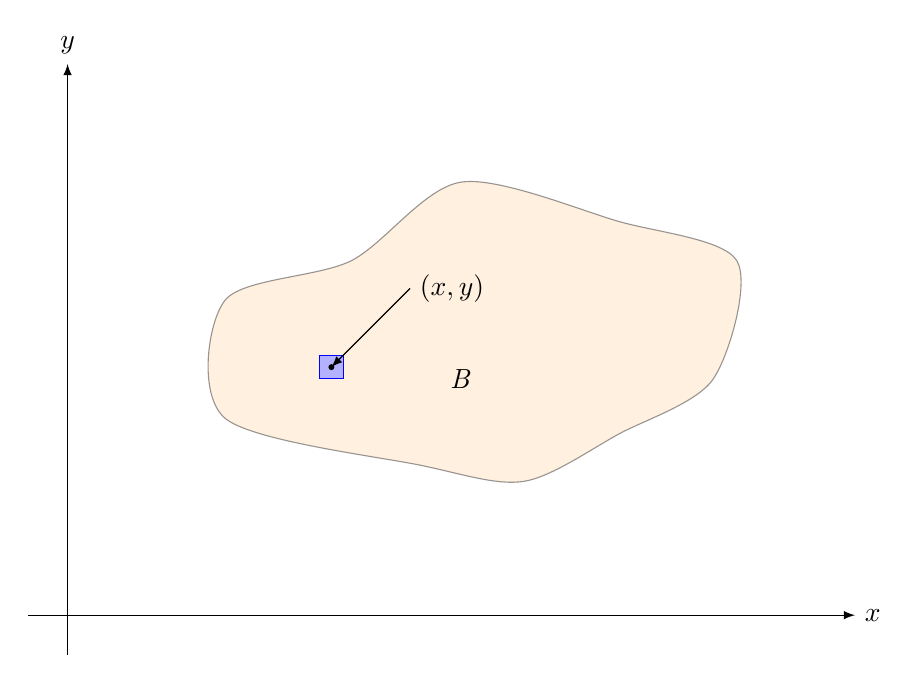
\begin{tikzpicture}
        \draw[-latex] (-0.5, 0) -- (10, 0) node[right] {$x$};
        \draw[-latex] (0, -0.5) -- (0, 7) node[above] {$y$};
        \draw[fill = orange!30, opacity = 0.4] plot [smooth cycle] 
        coordinates {(2, 2.5) (4.5, 1.9) (5.8, 1.7) (7, 2.3) (8.2, 3) 
        (8.5, 4.5) (7, 5) (5, 5.5) (3.6, 4.5) (2, 4)};
        \node[] at (5, 3) {\textit{B}};
        \draw[blue, fill = blue!30] (3.2, 3) rectangle (3.5, 3.3);
        \draw[fill = black] (3.35, 3.15) circle (0.03);
        \draw[latex-] (3.35, 3.15) -- (4.35, 4.15)  node[right] {$(x, y)$};
        
    \end{tikzpicture}
    \caption{A generic lamina that occupies the region \textit{B}}
    \label{fig:lamina}
\end{figure}

We can find the mass of the entire lamina by dividing it into many of these 
small rectangles and adding the masses of all the rectangles (see 
\ref{fig:laminagrid}). Just like in previous examples, there is some point 
$(x_{ij}^*, y_{ij}^*)$ in each rectangle, $R_{ij}$, such that the mass of the 
part of the lamina that occupies $R_{ij}$ is $\rho (x_{ij}^*, y_{ij}^*) \Delta 
A$. Adding all these masses yields:
$$m_{total} \approx \sum_{i = 1}^m \sum_{j = 1}^n \rho (x_{ij}^*, y_{ij}^*) 
\Delta A$$

Taking the limit as $m, n \to \infty$ increases the number of rectangles to 
yield the true total mass:
$$m_{total} = \lim_{m, n \to \infty} \sum_{i = 1}^m \sum_{j = 1}^n \rho (x_{ij
}^*, y_{ij}^*) \Delta A = \iint_{\textit{B}} \rho (x, y)\,dA$$

\begin{figure}[htbp]
\centering
    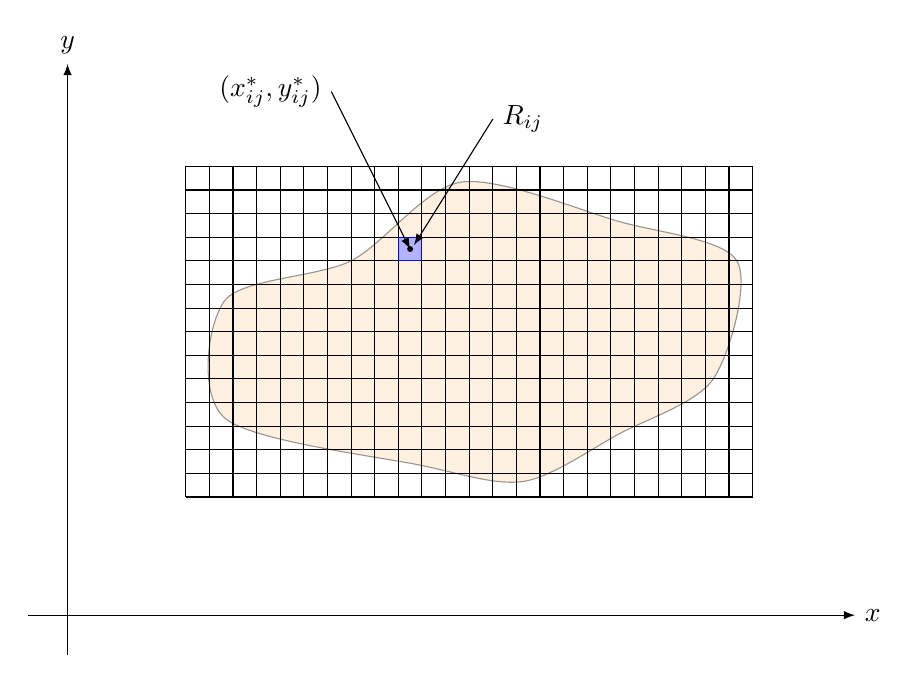
\begin{tikzpicture}
        \draw[-latex] (-0.5, 0) -- (10, 0) node[right] {$x$};
        \draw[-latex] (0, -0.5) -- (0, 7) node[above] {$y$};
        \draw[fill = orange!30, opacity = 0.4] plot [smooth cycle] 
        coordinates {(2, 2.5) (4.5, 1.9) (5.8, 1.7) (7, 2.3) (8.2, 3) 
        (8.5, 4.5) (7, 5) (5, 5.5) (3.6, 4.5) (2, 4)};
        \draw[step = 0.3] (1.5, 1.5) grid (8.7, 5.7);
        \draw[blue, fill = blue!30] (4.2, 4.5) rectangle (4.5, 4.8);
        \draw[fill = black] (4.35, 4.65) circle (0.03);
        \draw[latex-] (4.35, 4.65) -- (3.35, 6.65)  node[left] {$(x_{ij}^*, 
        y_{ij}^*)$};
        \draw[latex-] (4.4, 4.7) -- (5.4, 6.3) node[right] {$R_{ij}$};
        
    \end{tikzpicture}
    \caption{A generic lamina divided into many rectangles}
    \label{fig:laminagrid}
\end{figure}

\textbf{Example}: Find the total mass of a lamina that occupies the region 
$\textit{D} = \{ \left( x, y \right) \text{ }| \text{ } 1 \leq x \leq 3, 1 
\leq y \leq 4 \}$ with a density function $\rho (x, y) = 3y^2$. 

\textbf{Solution}: We know that the total mass is given by:
$$\iint_{\textit{D}} 3y^2\,dA$$

Applying Fubini's theorem, we see that:
$$\iint_{\textit{D}} 3y^2\,dA = \int_1^3 \int_1^4 3y^2\,dy\,dx$$
$$= \int_1^3 \left[ y^3 \right]_{y = 1}^{y = 4}\,dx = \int_1^3 \left[4^3 - 
1^3 \right]\,dx$$
$$= \int_1^3 63 \,dx = 63x|_{x = 1}^{x = 3} = 126$$

\begin{Exercise}[title = {Finding Total Mass}, label = total_mass]
Find the mass of the lamina that occupies the region, \textit{D}, and has the 
given density function, $\rho$. 
\begin{enumerate}
\item $\textit{D} = \{(x, y)\text{ }|\text{ } 0 \leq x \leq 4, 0 \leq y \leq 3 
\}; \rho (x, y) = 1 + x^2 + y^2$
\item \textit{D} is the triangular region with vertices $(0, 0)$, $(2, 1)$, 
$(0, 3)$; $\rho (x, y) = x + y$
\end{enumerate}
\end{Exercise}

\begin{Answer}[ref = total_mass]
\begin{enumerate}
    \item $\iint_{\textit{D}} \left(1 + x^2 + y^2 \right)\,dA = \int_0^4 
    \int_0^3 \left( 1  + x^2 + y^2 \right)\,dy\,dx$ $= \int_0^4 \left[y + x^2y 
    + \frac{1}{3}y^3 \right]_{y = 0}^{y = 3}\,dx$ $= \int_0^4 \left[ 3 + 3x^2 
    + \frac{1}{3}(3)^3 \right]\,dx$ $= \int_0^4 \left(12 + 3x^2 \right)\,dx$ 
    $= \left[ 12x + x^3 \right]_{x = 0}^{x = 4} = 12(4) + 4^3 = 112$
    \item First, let's visualize this region, since it isn't a rectangle:
    
    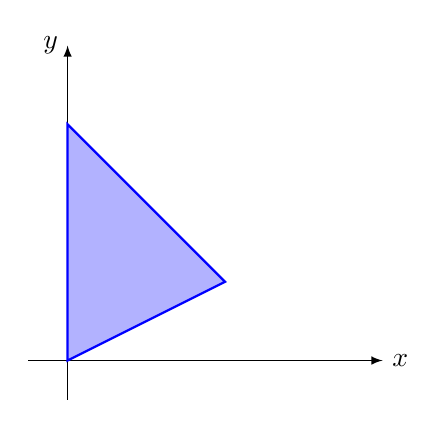
\begin{tikzpicture}
        \centering
        \draw[-latex] (-0.5, 0) -- (4, 0) node[right] {$x$};
        \draw[-latex] (0, -0.5) -- (0, 4) node[left] {$y$};
        \draw[thick, blue, fill = blue!30] (0,0) -- (2, 1) -- (0, 3) -- cycle;
    \end{tikzpicture}

    Let's divide the triangle horizontally and write equations for each of the 
    sides that do not lie on the $y$-axis.

    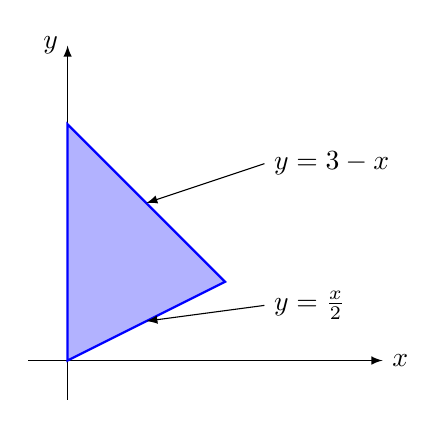
\begin{tikzpicture}
        \centering
        \draw[-latex] (-0.5, 0) -- (4, 0) node[right] {$x$};
        \draw[-latex] (0, -0.5) -- (0, 4) node[left] {$y$};
        \draw[thick, blue, fill = blue!30] (0,0) -- (2, 1) -- (0, 3) -- cycle;
        \draw[latex-] (1, 0.5) -- (2.5, 0.7) node[right] {$y = \frac{x}{2}$};
        \draw[latex-] (1, 2) -- (2.5, 2.5) node[right] {$y = 3 - x$};
    \end{tikzpicture}

    We see that we can describe region \textit{D} as $\textit{D} = \{ (x, y) 
    \text{ }|\text{ } 0 \leq x \leq 2, \frac{x}{2} \leq y \leq 3 - x\}$. 
    Therefore $\iint_{\textit{D}} \left( x + y \right) \,dA$ $= \int_0^3 \int_{
    x/2}^{3 - x} \left(x + y \right)\,dy\,dx$ $= \int_0^3 \left[xy + 
    \frac{1}{2} y^2 \right]_{y = x/2}^{y = 3 - x}\,dx$ $= \int_0^3 \left[ 
    \left(x(3 - x) \right) - \left(x (x/2) \right) + \frac{1}{2} \left( (3 - 
    x)^2 - (x/2)^2 \right) \right]\,dx$ $= \int_0^3 \left[ \left(3x - x^2 - 
    \frac{x^2}{2} \right) + \frac{1}{2} \left( 9 - 6x + x^2 - \frac{x^2}{4} 
    \right) \right]\,dx$ $= \int_0^3 \left[-x^2 - \frac{x^2}{2} + \frac{x^2}{2}
    - \frac{x^2}{8} + 3x - 3x + \frac{9}{2} \right]\,dx$ $= \int_0^3 \left( -
    \frac{9x^2}{8} + \frac{9}{2} \right)\,dx$ $= \left[ \frac{9x}{2} -\frac{
    3x^3}{8} \right]_{x = 0}^{x = 2}$ $= \frac{9(2)}{2} - \frac{3(8)}{8} = 9 - 
    3 = 6$
\end{enumerate}
\end{Answer}

This method applies not only to mass density, but any other type of density. 
Some examples could include animals per acre of forest, cells per square 
centimeter of petri dish, or people per city block. A density physicists are 
often interested in is charge density (that is, the amount of charge, $Q$, per 
unit area). Charge is measured in coulombs (C). Often, charge density is given 
by a function, $\sigma (x, y)$, in units of coulombs per area (such as 
$\text{cm}^2$ or $\text{m}^2$). If there is some region, \textit{D}, with 
charge distributed across it such that the charge density can be described 
by a continuous function, $\sigma (x, y)$, then the total charge, Q, is given 
by:
$$Q = \iint_{\textit{D}} \sigma (x, y)\,dA$$

\textbf{Example}: Charge is distributed over the region \textit{B} shown in 
figure \ref{fig:charge} such that the charge density is given by $\sigma (x, y)
= xy$, measured in C/$\text{m}^2$. Find the total charge. 

\begin{figure}[htbp]
\centering
    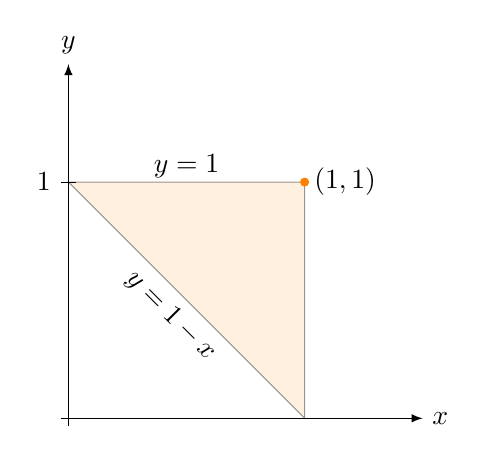
\begin{tikzpicture}
        \draw[-latex] (-0.1, 0) -- (4.5, 0) node[right] {$x$};
        \draw[-latex] (0, -0.1) -- (0, 4.5) node[above] {$y$};
        \draw[fill = orange!30, opacity = 0.4] (3, 0) -- (3, 3) -- (0, 3) -- 
        cycle;
        \draw[orange, fill = orange] (3, 3) circle (0.05) node[black, right] 
        {$(1, 1)$};
        \draw[] (0.1, 3) -- (-0.1, 3) node[left] {$1$};
        \node[] at (1.5, 3.2) {$y = 1$};
        \node[rotate = -45] at (1.3, 1.3) {$y = 1 - x$};
        
    \end{tikzpicture}
    \caption{A triangular region over which charge is distributed such that 
    $\sigma (x, y) = xy$}
    \label{fig:charge}
\end{figure}

\textbf{Solution}: We know that total charge is given by:
$$Q = \iint_{\textit{B}} xy\,dA$$ 

Examining figure \ref{fig:charge}, we see that:
$$\iint_{\textit{B}} xy\,dA = \int_0^1 \int_{1 - x}^1 xy\,dy\,dx$$
$$= \int_0^1 \frac{x}{2} \left[ y^2 \right]_{y = 1 - x}^{y = 1}\,dx = \int_0^1 
\frac{x}{2} \left[ 1^2 - \left( 1 - x \right)^2 \right]\,dx$$
$$= \frac{1}{2} \int_0^1 x \left(1 - 1 + 2x - x^2 \right)\,dx = \frac{1}{2} 
\int_0^1 x \left(2x - x^2 \right)\,dx$$
$$= \frac{1}{2} \int_0^1 2x^2 - x^3\,dx = \frac{1}{2} \left[ \frac{2}{3}x^3 - 
\frac{1}{4}x^4 \right]_{x = 0}^{x = 1} = \frac{1}{2} \left( \frac{2}{3} - 
\frac{1}{4} \right) = \frac{5}{24} \text{C}$$


\section{Center of Mass}
For a thin disk (lamina) of variable density in the $xy$-plane, the coordinates
of the center of mass, $(\overline{x}, \overline{y})$, are given by:
$$\overline{x} = \frac{1}{m} \iint_{\textit{D}} x \rho (x, y)\,dA$$
$$\overline{y} = \frac{1}{m} \iint_{\textit{D}} y \rho (x, y)\,dA$$

Where $m$ is the total mass and $\rho$ is the density of the lamina as a 
function of $x$ and $y$. 

\textbf{Example}: Find the center of mass of a triangular lamina with vertices 
at $(0, 0)$, $(2, 0)$, and $(0, 1)$ and a density function $\rho (x, y) = 2 + 
x + 3y$. 

\textbf{Solution}: We begin by visualizing the region so we can determine if 
it is type I or type II:

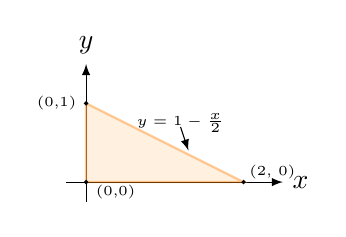
\begin{tikzpicture}
    \draw[-latex] (-0.25, 0) -- (2.5, 0) node[right] {$x$};
    \draw[-latex] (0, -0.25) -- (0, 1.5) node[above] {$y$};
    \draw[orange, thick, fill = orange!30, opacity = 0.4] (0,0) -- (2, 0) -- 
    (0, 1) -- cycle;
    \node[font = \tiny] at (1.2, 0.75) {$y = 1 - \frac{x}{2}$};
    \draw[-latex] (1.2, 0.7) -- (1.3, 0.4);
    \draw[black, fill = black] (0,1) circle (0.02cm) node[font = \tiny, left] 
    {(0,1)};
    \draw[black, fill = black] (0,0) circle (0.02cm) node[font = \tiny, right, 
    yshift = -0.13cm] {(0,0)};
    \draw[black, fill = black] (2, 0) circle (0.02cm) node[font = \tiny, right, 
    yshift = 0.13cm, xshift = -0.05cm] {(2, 0)};
\end{tikzpicture}

Recall that the total mass is given by $m = \iint_{\textit{D}} \rho (x, y)
\,dA$. As shown above, we can define $\textit{D} = \{ \left( x, y \right) | 0 
\leq x \leq 2, 0 \leq y \leq 1 - \frac{x}{2} \}$:
$$m = \int_{0}^{2} \int_{0}^{1 - x/2} \left( 2 + x + 3y \right) \,dy \,dx = 
\int_{0}^2 \left[2y + xy + \frac{3}{2}y^2 \right]_{y = 0}^{y = 1 - x/2}\,dx$$
$$= \int_0^2 \left[ 2(1 - \frac{x}{2}) + x(1 - \frac{x}{2}) + \frac{3}{2} (1 - 
\frac{x}{2})^2 \right]\,dx = \int_0^2 \left[ \frac{7}{2} - \frac{3x}{2} - 
\frac{x^2}{8} \right]\,dx$$
$$= \left[ \frac{7x}{2} - \frac{3x^2}{4} - \frac{x^3}{24} \right]_{x = 0}^{x = 
2} = \frac{7(2)}{2} - \frac{3(4)}{4} - \frac{8}{24} = 7 - 3 - \frac{1}{3} = 
\frac{11}{3}$$

Finding $\overline{x}$:
$$\overline{x} = \frac{1}{m} \iint_{\textit{D}} x \left( 2 + x + 3y \right) 
\,dA$$
$$\overline{x} = \frac{3}{11} \int_0^2 \int_0^{1 - x/2} \left[ 2x + x^2 + 3xy 
\right] \,dy \,dx$$
$$\overline{x} = \frac{3}{11} \int_0^2 \left[ 2xy + x^2y + \frac{3}{2}xy^2 
\right]_{y = 0}^{y = 1 - x/2} \,dx$$
$$\overline{x} = \frac{3}{11} \int_0^2 \left[ \frac{7x}{2} - \frac{3x^2}{2} - 
\frac{x^3}{8} \right]\,dx$$
$$\overline{x} = \frac{3}{11} \left[ \frac{7x^2}{4} - \frac{x^3}{2} - \frac{x
^4}{32} \right]_{x = 0}^{x = 2}$$
$$\overline{x} = \frac{3}{11} \left[ \frac{7(4)}{4} - \frac{8}{2} - \frac{16}{
32} \right] = \frac{3}{11} \left( 7 - 4 - \frac{1}{2} \right) = \frac{3}{11} 
\left( \frac{5}{2} \right) = \frac{15}{22}$$

And we can similarly find $\overline{y}$:
$$\overline{y} = \frac{1}{m} \iint_{\textit{D}} y \left(2 + x + 3y \right)
\,dA$$
$$\overline{y} = \frac{3}{11} \int_0^2 \int_0^{1 - x/2} \left[ 2y + xy + 3y^2 
\right]\,dy\,dx$$
$$\overline{y} = \frac{3}{11} \int_0^2 \left[ y^2 + \frac{x}{2}y^2 + y^3 
\right]_{y = 0}^{y = 1 - x/2} \,dx$$
$$\overline{y} = \frac{3}{11} \int_0^2 \left[ \left(1 - \frac{x}{2} \right)^2 
+ \frac{x}{2} \left( 1 - \frac{x}{2} \right)^2 + \left( 1 - \frac{x}{2} \right)
^3 \right] \,dx$$
$$\overline{y} = \frac{3}{11} \int_0^2 \left[ 2 - 2x + \frac{x^2}{2} \right]
\,dx = \frac{3}{11} \left[ 2x - x^2 + \frac{x^3}{6} \right]_{x = 0}^{x = 2}$$
$$\overline{y} = \frac{3}{11} \left[ 2(2) - 2(2) + \frac{8}{6} \right] = \frac{
3}{11} \left( \frac{4}{3} \right) = \frac{4}{11}$$

Therefore, the center of mass $(\overline{x}, \overline{y})$ is $(\frac{15}{22
}, \frac{4}{11})$.

\begin{Exercise}[title = {Center of Mass}, label = c_of_m]
Find the center of mass of 
\begin{enumerate}
\item a lamina that occupies the area enclosed by the 
curves $y = 0$ and $y = 2\sin{x}$ from $0 \leq x \leq \pi$ if its density is 
given by $\rho (x,y) = x$.
\item the region \textit{D} if $\textit{D} = \{(x, y)\text{ }|\text{ } 0 \leq x
\leq 4, 0 \leq y \leq 3 \}; \rho (x, y) = 1 + x^2 + y^2$
\item The triangular region \textit{D} with vertices $(0, 0)$, $(2, 1)$, 
$(0, 3)$; $\rho (x, y) = x + y$
\end{enumerate}
\vspace{100mm}
\end{Exercise}

\begin{Answer}[ref = c_of_m]
\begin{enumerate}
\item First, we find the total mass: $m = \int_0^{\pi} \int_0^{2\sin{x}} x \,dy
\,dx$ 
$= \int_0^{\pi} \left[ xy \right]_{y = 0}^{y = 2\sin{x}}\,dx$ $= \int_0^{\pi} 2
x\sin{x}\,dx$. 

We apply integration by parts to evaluate the integral: 
$\int_0^{\pi} 2x\sin{x}\,dx = \left(-2x \cos{x} \right)|_{x = 0}^{x = \pi} + 
\int_0^{\pi} 2 \cos{x}\,dx$ 
$= \left[-2 \pi (-1) \right] - \left( 0 \right) + \sin{x}|_{x = 0}^{x = \pi}$ 
$= 2\pi + \sin{\pi} - \sin{0} = 2\pi$

Now that we know $m = 2\pi$, we can find $\overline{x}$ and $\overline{y}$: 
$\overline{x} = \frac{1}{2\pi} \int_0^{\pi} \int_0^{2\sin{x}} x \cdot x \,dy 
\,dx$ 
$= \frac{1}{2\pi} \int_0^{\pi} x^2y|_{y = 0}^{y = 2\sin{x}}\,dx$ 
$= \frac{1}{2\pi} \int_0^{\pi} x^2 \left(2\sin{x} \right)\,dx$ 
$= \frac{1}{\pi} \int_0^{\pi} x^2 \sin{x}\,dx$. 

Applying integration by parts: $\frac{1}{\pi} \int_0^{\pi} x^2 \sin{x}\,dx$ 
$= \frac{1}{\pi} \left[ x^2 \left(-\cos{x} \right)|_{x = 0}^{x = \pi} - \int_0^
{\pi} 2x \left( -\cos{x} \right) \,dx \right]$ 
$= \frac{1}{\pi} \left[ \left( -\pi^2 \cos{\pi} \right) + 2\int_0^{\pi} x\cos{x
}\,dx \right]$ 
$= \frac{1}{\pi} \left[ \pi^2 + 2\int_0^{\pi} x\cos{x}\,dx \right]$ $= \pi + 
\frac{2}{\pi} \int_0^{\pi} x\cos{x}\,dx$. 

Applying integration by parts again: $\pi + \frac{2}{\pi} \int_0^{\pi} x\cos{x}
\,dx$ 
$= \pi + \frac{2x\sin{x}}{\pi}|_{x = 0}^{x = \pi} - \frac{2}{\pi} \int_0^{\pi} 
\sin{x}\,dx$
$= \pi -\frac{2}{\pi} \int_0^{\pi} \sin{x}\,dx$
$= \pi + \frac{2}{\pi} \left[ \cos{x} \right]_{x = 0}^{x = \pi}$
$= \pi + \frac{2}{\pi} \left[ \cos{\pi} - \cos{0} \right]$
$= \pi + \frac{2}{\pi} \left(-1 - 1 \right)$ $= \pi - \frac{4}{\pi} = 
\overline{x}$

And finding $\overline{y}$: 
$\overline{y} = \frac{1}{2\pi} \int_0^{\pi} \int_0^{2 \sin{x}} y \cdot x \,dy 
\,dx$
$= \frac{1}{2\pi} \int_0^{\pi} \left[ \frac{1}{2}xy^2 \right]_{y = 0}^{y = 2
\sin{x}} \,dx$
$= \frac{1}{4\pi} \int_0^{\pi} x \left[ 2\sin{x} \right]^2 \,dx$ 
$= \frac{1}{4\pi} \int_0^{\pi} 4x \sin^2{x}\,dx$ 
$= \frac{1}{\pi} \int_0^{\pi} x\sin^2{x}\,dx$ 
$=\frac{1}{\pi} \int_0^{\pi} x \frac{1-\cos{\left(2x\right)}}{2}\,dx$ 
$= \frac{1}{\pi} \int_0^{\pi} \frac{x}{2}\,dx - \frac{1}{\pi} \int_0^{\pi} x 
\cos{(2x)}\,dx$ 
$= \frac{1}{2\pi} \left[ \frac{x^2}{2} \right]_{x = 0}^{x = \pi} - \frac{1}{\pi
} \left[ \frac{1}{2}x\sin{(2x)}|_{x = 0}^{x = \pi} - \frac{1}{2} \int_0^{\pi} 
\sin{(2x)}\,dx \right]$
$= \frac{1}{2\pi} \left( \frac{\pi^2}{2} \right) - \frac{1}{2\pi} \left[ \pi
\sin{(2\pi)} - 0 + \frac{1}{2} \cos{(2x)}|_{x - 0}^{x = \pi} \right]$
$= \frac{\pi}{4} - \frac{1}{2\pi} \left[ \frac{1}{2} \left(\cos{2\pi} - \cos{0}
\right) \right] = \frac{\pi}{4}$

And therefore the center of mass is found at $\left( \overline{x}, \overline{y}
\right) = \left( \pi - \frac{4}{\pi}, \frac{\pi}{4} \right)$

\item We know from a previous question that the total mass of this lamina is 
112 (see \textit{Finding Total Mass}). 

Finding $\overline{x}$: $\overline{x} = \frac{1}{112} \int_0^4 \int_0^3 x 
\left( 1 + x^2 + y^2 \right)\,dy\,dx$ 
$= \frac{1}{112} \int_0^4 \int_0^3 \left(x + x^3 + xy^2 \right)\,dy\,dx$ 
$= \frac{1}{112} \int_0^4 \left[ xy + x^3y + \frac{x}{3}y^3 \right]_{y = 0}^{y 
= 3} \,dx$ 
$= \frac{1}{112} \int_0^4 \left[3x + 3x^3 + 9x \right]\,dx$ 
$= \frac{3}{112} \int_0^4 \left[ 4x + x^3 \right]\,dx$ 
$= \frac{3}{112} \left[ 2x^2 + \frac{x^4}{4} \right]_{x = 0}^{x = 4}$ 
$= \frac{3}{112} \left[ 2(4)^2 - 2(0)^2 + \frac{4^4}{4} - \frac{0^4}{4} 
\right]$ 
$= \frac{3}{112} \left[ 32 + 64 \right] = \frac{3 \cdot 96}{112} = \frac{3 
\cdot 2 \cdot 2 \cdot 2 \cdot 2 \cdot 2 \cdot 3}{2 \cdot 2 \cdot 7 \cdot 2 
\cdot 2} = \frac{18}{7}$

Finding $\overline{y}$: $\overline{y} = \frac{1}{112} \int_0^4 \int_0^3 y 
\left( 1 + x^2 + y^2 \right)\,dy\,dx$ 
$= \frac{1}{112} \int_0^4 \int_0^3 \left[ y + x^2y + y^3 \right]\,y\,dx$ 
$= \frac{1}{112} \int_0^4 \left[ \frac{y^2}{2} + \frac{x^2y^2}{2} + \frac{y^4}{
4} \right]_{y = 0}^{y = 3} \,dx$ 
$= \frac{1}{112} \int_0^4 \left[ \frac{3^2}{2} + \frac{3^2x^2}{2} + \frac{3^4}{
4} \right]\,dx$ 
$= \frac{1}{112} \int_0^4 \left[ \frac{99}{4} + \frac{9}{2}x^2 \right] \,dx$ 
$= \frac{1}{112} \left[ \frac{99}{4}x + \frac{3}{2}x^3 \right]_{x = 0}^{x = 4}$ 
$= \frac{3}{224} \left[\frac{33}{2}(4) + 4^3 \right]$ 
$= \frac{3}{224} \left( 66 + 64 \right) = \frac{3 \cdot 130}{224} = \frac{3 
\cdot 65}{112} = \frac{195}{112}$

Therefore the center of mass of the rectangular region \textit{D} is $\left(
\frac{18}{7}, \frac{195}{112} \right)$

\item We know from a previous question (see \textit{Finding Total Mass}) that 
the total mass of \textit{D} is 6 and it can be described as $\textit{D} = \{ (
x, y) \text{ }|\text{ } 0 \leq x \leq 2, \frac{x}{2} \leq y \leq 3 - x\}$

Finding $\overline{x}$:

$\overline{x} = \frac{1}{6} \int_0^2 \int_{x/2}^{3 - x} x \left(x + y \right)
\,dy\,dx$
$= \frac{1}{6} \int_0^2 \int_{x/2}^{3 - x} \left(x^2 + xy \right)\,dy\,dx$
$= \frac{1}{6} \int_0^2 \left[ x^2y + \frac{x}{2}y^2 \right]_{y = x/2}^{y = 3 -
x}\,dx$
$= \frac{1}{6} \int_0^2 \left[ x^2\left( 3 - x - \frac{x}{2} \right) + \frac{x
}{2}\left( \left( 3 - x \right)^2 - \left( \frac{x}{2} \right)^2 \right) 
\right]\,dx$
$= \frac{1}{6} \int_0^2 \left[ 3x^2 - x^3 - \frac{x^3}{2} + \frac{x}{2} \left(
9 - 6x + x^2 - \frac{x^2}{4} \right) \right]\,dx$
$= \frac{1}{6} \int_0^2 \left[ 3x^2 - \frac{3}{2}x^3 + \frac{x}{2} \left( 9 - 
6x + \frac{3}{4}x^2 \right) \right]\,dx$
$= \frac{1}{6} \int_0^2 \left[ 3x^2 - \frac{3}{2}x^3 + \frac{9}{2}x - 3x^2 + 
\frac{3}{8}x^3 \right]\,dx$
$= \frac{1}{6} \int_0^2 \left[ \frac{9}{2}x - \frac{9}{8}x^3 \right]\,dx$
$= \frac{1}{6} \left[ \frac{9}{4}x^2 - \frac{9}{32}x^4 \right]_{x = 0}^{x = 2}$
$= \frac{1}{6} \left[ \frac{9 \cdot 4}{4} - \frac{9 \cdot 16}{32} \right]$
$= \frac{1}{6} \left[9 - \frac{9}{2} \right] = \frac{1}{6} \cdot \frac{9}{2} = 
\frac{9}{12} = \frac{3}{4}$

And finding $\overline{y}$:

$\overline{y} = \frac{1}{6} \int_0^2 \int_{x/2}^{3 - x} y \left(x + y \right)
\,dy\,dx$
$= \frac{1}{6} \int_0^2 \int_{x/2}^{3-x} \left(xy + y^2 \right)\,dy\,dx$
$= \frac{1}{6} \int_0^2 \left[ \frac{x}{2}y^2 + \frac{1}{3}y^3 \right]_{y = x/2
}^{y = 3 - x}\,dx$
$= \frac{1}{6} \int_0^2 \left[ \frac{x}{2} \left( \left( 3 - x \right)^2 - 
\left( \frac{x}{2} \right)^2 \right) + \frac{1}{3} \left( \left( 3 - x \right)^
3 - \left( \frac{x}{2} \right)^3 \right) \right]\,dx$
$= \frac{1}{6} \int_0^2 \left[ \frac{x}{2} \left( 9 - 6x + x^2 - \frac{x^2}{4} 
\right) + \frac{1}{3} \left( 27 - 27x +9x^2 - x^3 - \frac{x^3}{8} \right) 
\right]\,dx$
$= \frac{1}{6} \int_0^2 \left[ \frac{x}{2} \left( 9 - 6x + \frac{3x^2}{4} 
\right) + \frac{1}{3} \left( 27 - 27x + 9x^2 - \frac{9x^3}{8} \right) \right]
\,dx$
$= \frac{1}{6} \int_0^2 \left[ \frac{9}{2}x - 3x^2 + \frac{3}{8}x^3 + 9 - 9x + 
3x^2 - \frac{3}{8}x^3 \right]\,dx$
$= \frac{1}{6} \int_0^2 \left[ 9 - \frac{9}{2}x  \right]\,dx$
$= \frac{1}{6} \left[ 9x - \frac{9}{4}x^2 \right]_{x = 0}^{x = 2}$
$= \frac{3}{6} \left[3(2) - \frac{3}{4}(2)^2 \right]$
$= \frac{1}{2} \left(6 - 3 \right) = \frac{1}{2} \cdot 3 = \frac{3}{2}$

Therefore, the center of mass is $\left( \overline{x}, \overline{y} \right) = 
\left( \frac{3}{4}, \frac{3}{2} \right)$
\end{enumerate}

\end{Answer}

\section{Moment of Inertia}

\section{Surface Area}